\documentclass[12pt]{article}
%--------------------   start of the 'preamble'
%
\usepackage{graphicx,amssymb,amstext,amsmath,color}
\usepackage[margin=2cm]{geometry}
\usepackage{abstract}
\usepackage{setspace}
\usepackage[footnotesize,bf]{caption}

% TABLE
\usepackage{multicol,hhline,colortbl,multirow,adjustbox}
\usepackage{braket}
\usepackage{siunitx}
\usepackage{hyperref}
\usepackage{authblk}
\usepackage{siunitx}
\usepackage{mathrsfs}
%%\usepackage[sort&compress]{natbib}
%%\bibpunct{(}{)}{,}{a}{, }{;}
%
\usepackage[sort&compress]{natbib}
\bibpunct{[}{]}{,}{s}{}{;}


\definecolor{gray}{gray}{0.8}
\def\mobunits{\square\centi\meter\per\volt\per\second}
\def\gcm{\gram\per\cubic\centi\meter}
\def\ccg{\cellcolor{gray}}

\renewcommand{\labelitemii}{$\circ$}
\renewcommand{\bibname}{References}


\title{MorphCT - 1K P3HT 15mers}
\author{Matthew Jones}
\date{\today}

\begin{document}
\maketitle


\section{Simulations}


The simulations for the systems containing 1,000 15mers of P3HT have completed.
There are 4 systems.
Those labelled `ordered', `disordered', and `semicrystalline' have been assigned based on the visual order/disorder of the system - no quantification of the level of order has been performed, so these names are subject to change as more data is obtained.
The final system contains a blend of p3ht-pcbm. 
For now, only the hole transport properties are of interest and so reported in this document.


NOTE: The recent improvements in the functionality of MorphCT (namely, Koopmans' approximation, VRH and simple energy penalties for hopping) were developed after these systems were submitted and so have not been included here.
Any combination of these additional mechanisms could dramatically change the resultant mobilities in any number of ways.


\section{Observations}

\begin{itemize}
    \item{The number of stacks is a good metric for (at least visual) crystalline order}
    \item{Intercalating PCBM increases the number of stacks (as expected)}
    \item{Without Koopmans, VRH, or some other mechanism, the mobility-order trend is not replicated (ordered and disordered have the same mobility, semicrystalline is an order of magnitude lower. We would expect a monotonic decrease across the three).}
\end{itemize}

\section{Mobility Results}

\begin{center}
\begin{adjustbox}{max width = \textwidth}
\begin{tabular}{| c | c | c | c | c | c |}
\hline
\rule{0pt}{2.5ex} 
\multirow{2}{*}{\textbf{Simulation Name}}&\textbf{Density}&\textbf{Anisotropy}&\textbf{Stacks}&\textbf{Stack Threshold}&\textbf{Hole Mobility}\\
                            &(\SI{}{\gcm})&(Arb. U.)&(Arb. U.)&(\AA)&(\SI{}{\mobunits})\\
\hhline{|======|}
{\ccg}\rule{0pt}{2.5ex}large\_p3ht\_ordered&{\ccg}---&{\ccg}0.1375&{\ccg}12&{\ccg}4.00&{\ccg}2.99$\times 10^{0}$\\
\rule{0pt}{2.5ex}large\_p3ht\_semicrystalline&---&0.0175&24&4.00&4.29$\times 10^{-1}$\\
{\ccg}\rule{0pt}{2.5ex}large\_p3ht\_disordered&{\ccg}---&{\ccg}0.0007&{\ccg}38&{\ccg}4.00&{\ccg}3.02$\times 10^{0}$\\
\rule{0pt}{2.5ex}large\_p3ht\_pcbm&---&0.0775&43&4.00&1.47$\times 10^{0}$\\
\hhline{------}
\end{tabular}\label{table:mob}
\end{adjustbox}
\captionof{table}{The results from MorphCT.}
\end{center}


\clearpage


\begin{figure}[h]\centering
	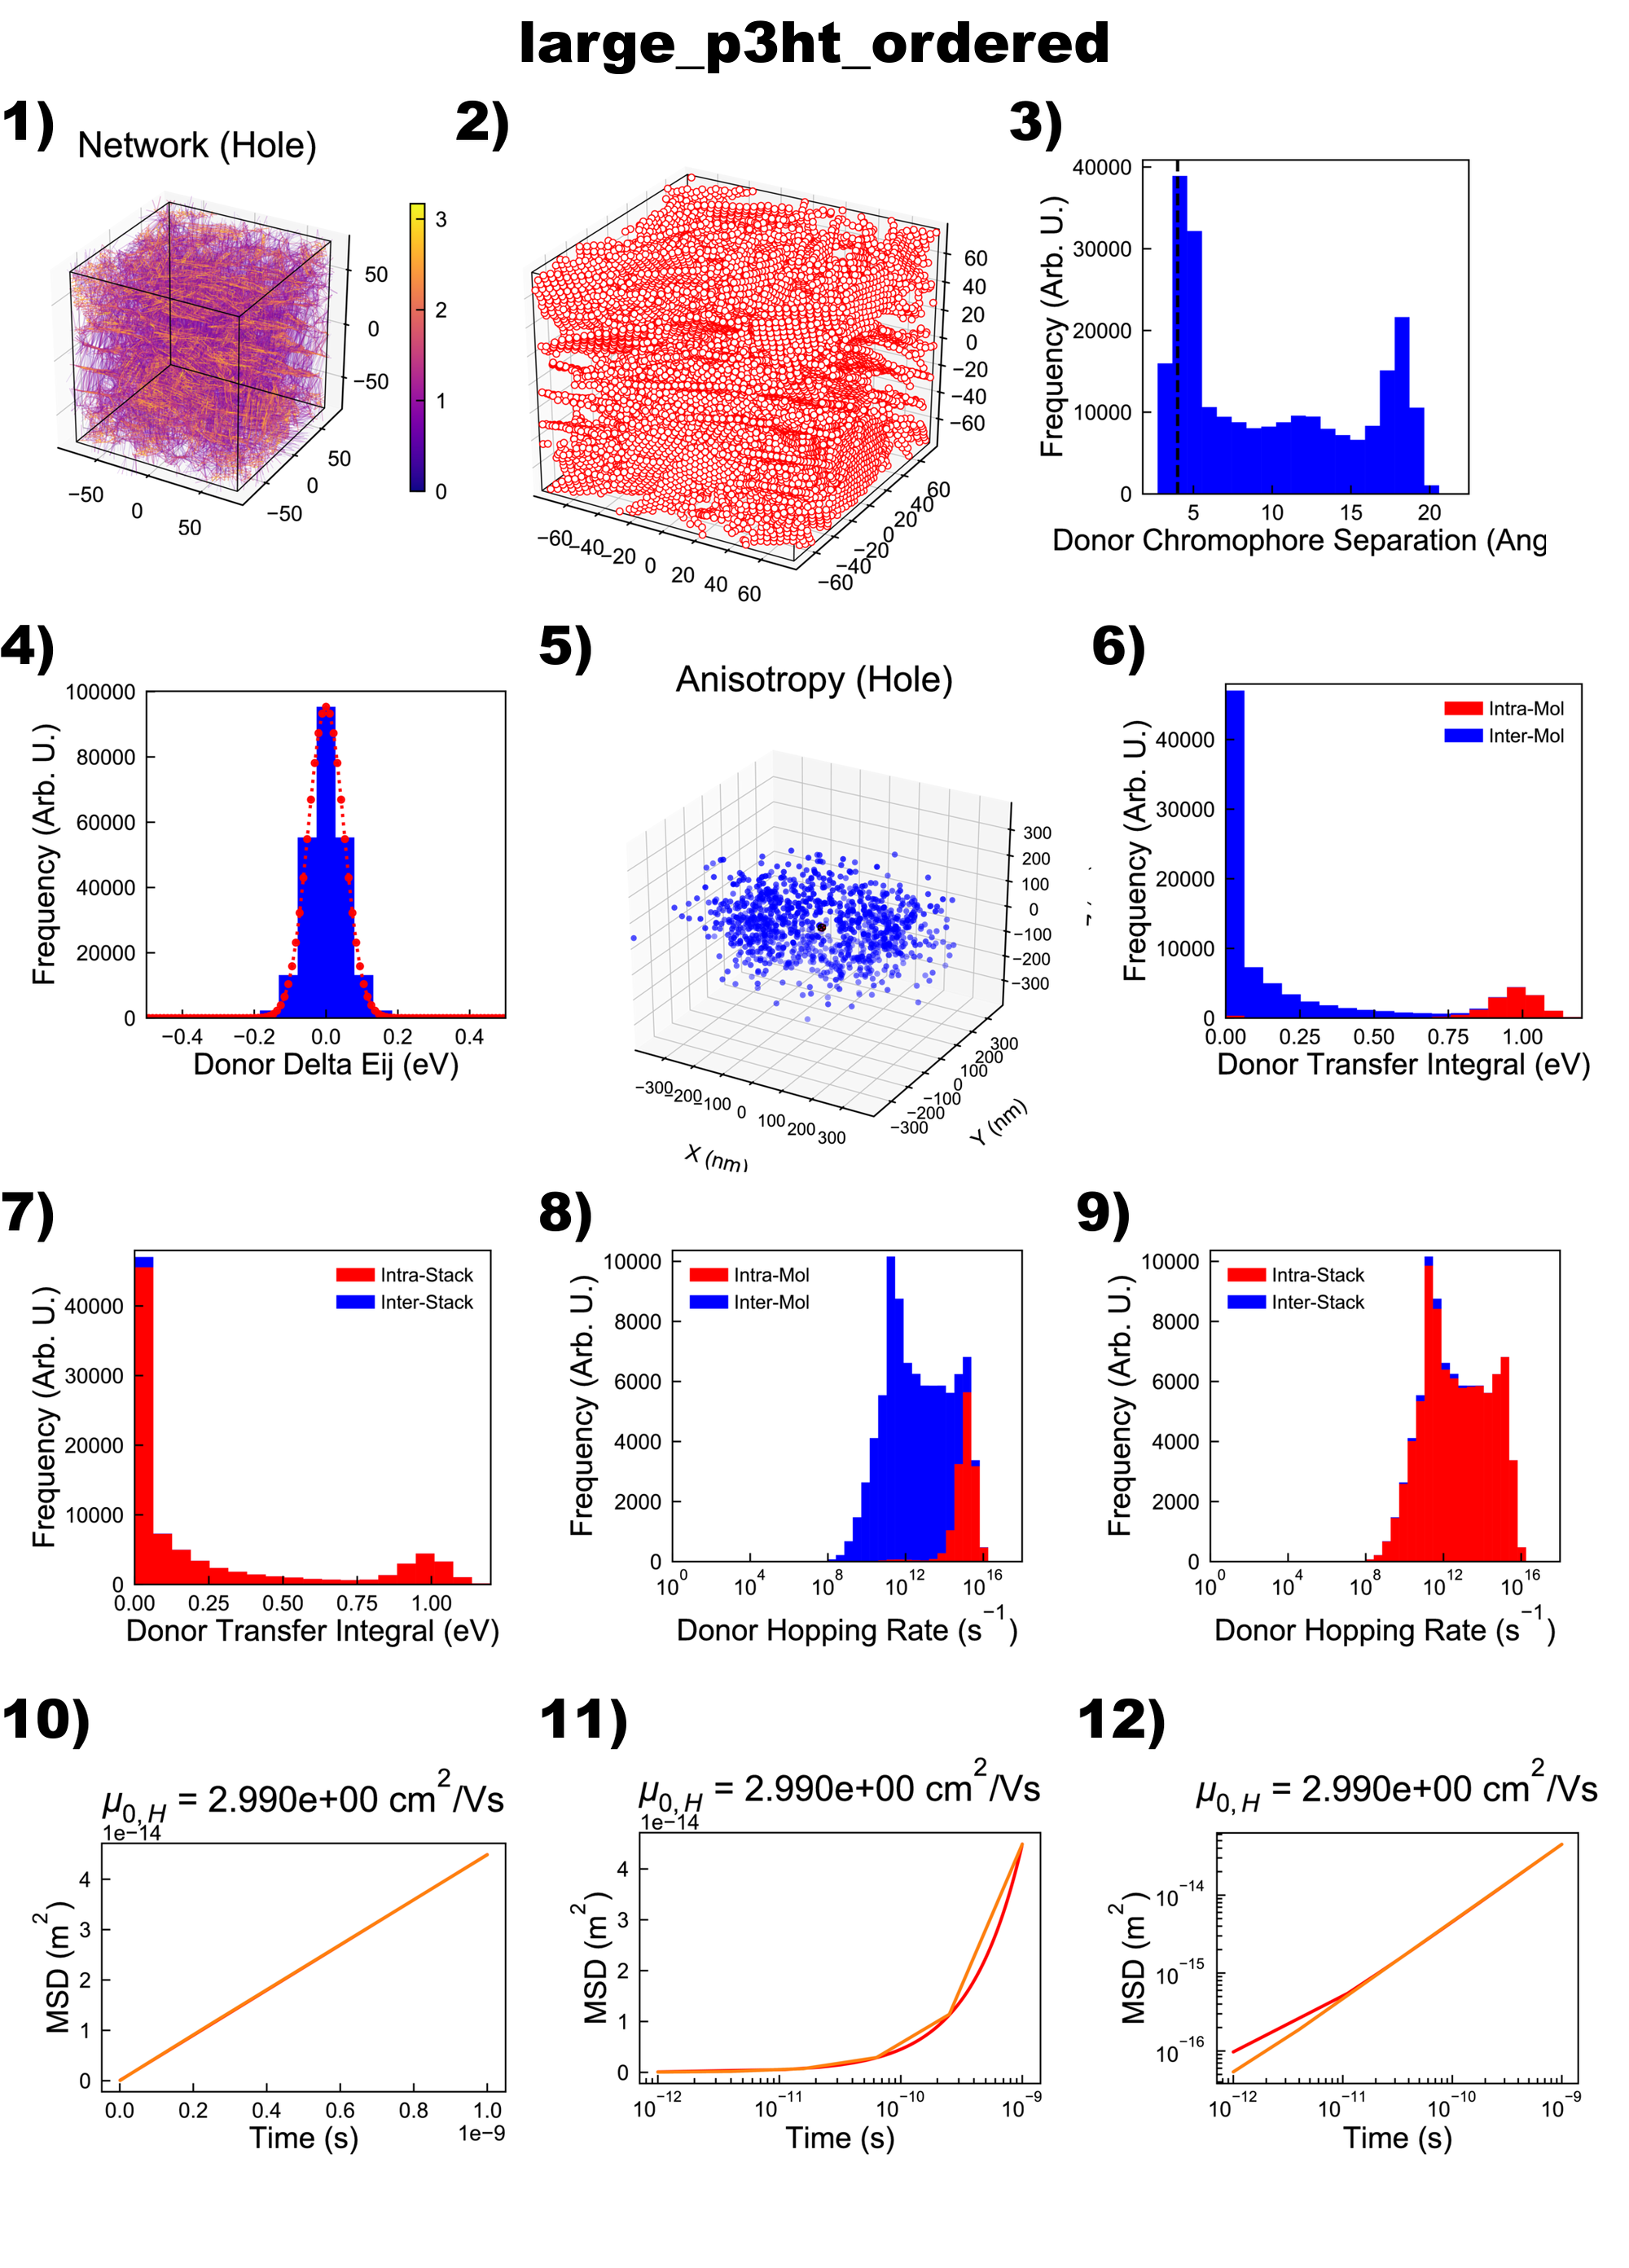
\includegraphics[width=0.85\textwidth]{Figures/large_p3ht_ordered.png}
    \caption{   1) Chromophore connectivity network, 
                2) Location of `stacks', 
                3) Distribution of connected chromophore separations (defines stacks),
                4) Density of states of Frontier molecular orbital (delta Eij),
                5) KMC Carrier termination locations (defines anisotropy),
                6) Histogram of molecular transfer integrals,
                7) Histogram of stack transfer integrals,
                8) Histogram of molecular hopping rates,
                9) Histogram of stack hopping rates,
                10) Linear MSD plot,
                11) Semi-log-x MSD plot,
                12) Logarithmic MSD plot.}
	\label{fig:largeOrdered}
\end{figure}


\begin{figure}[h]\centering
	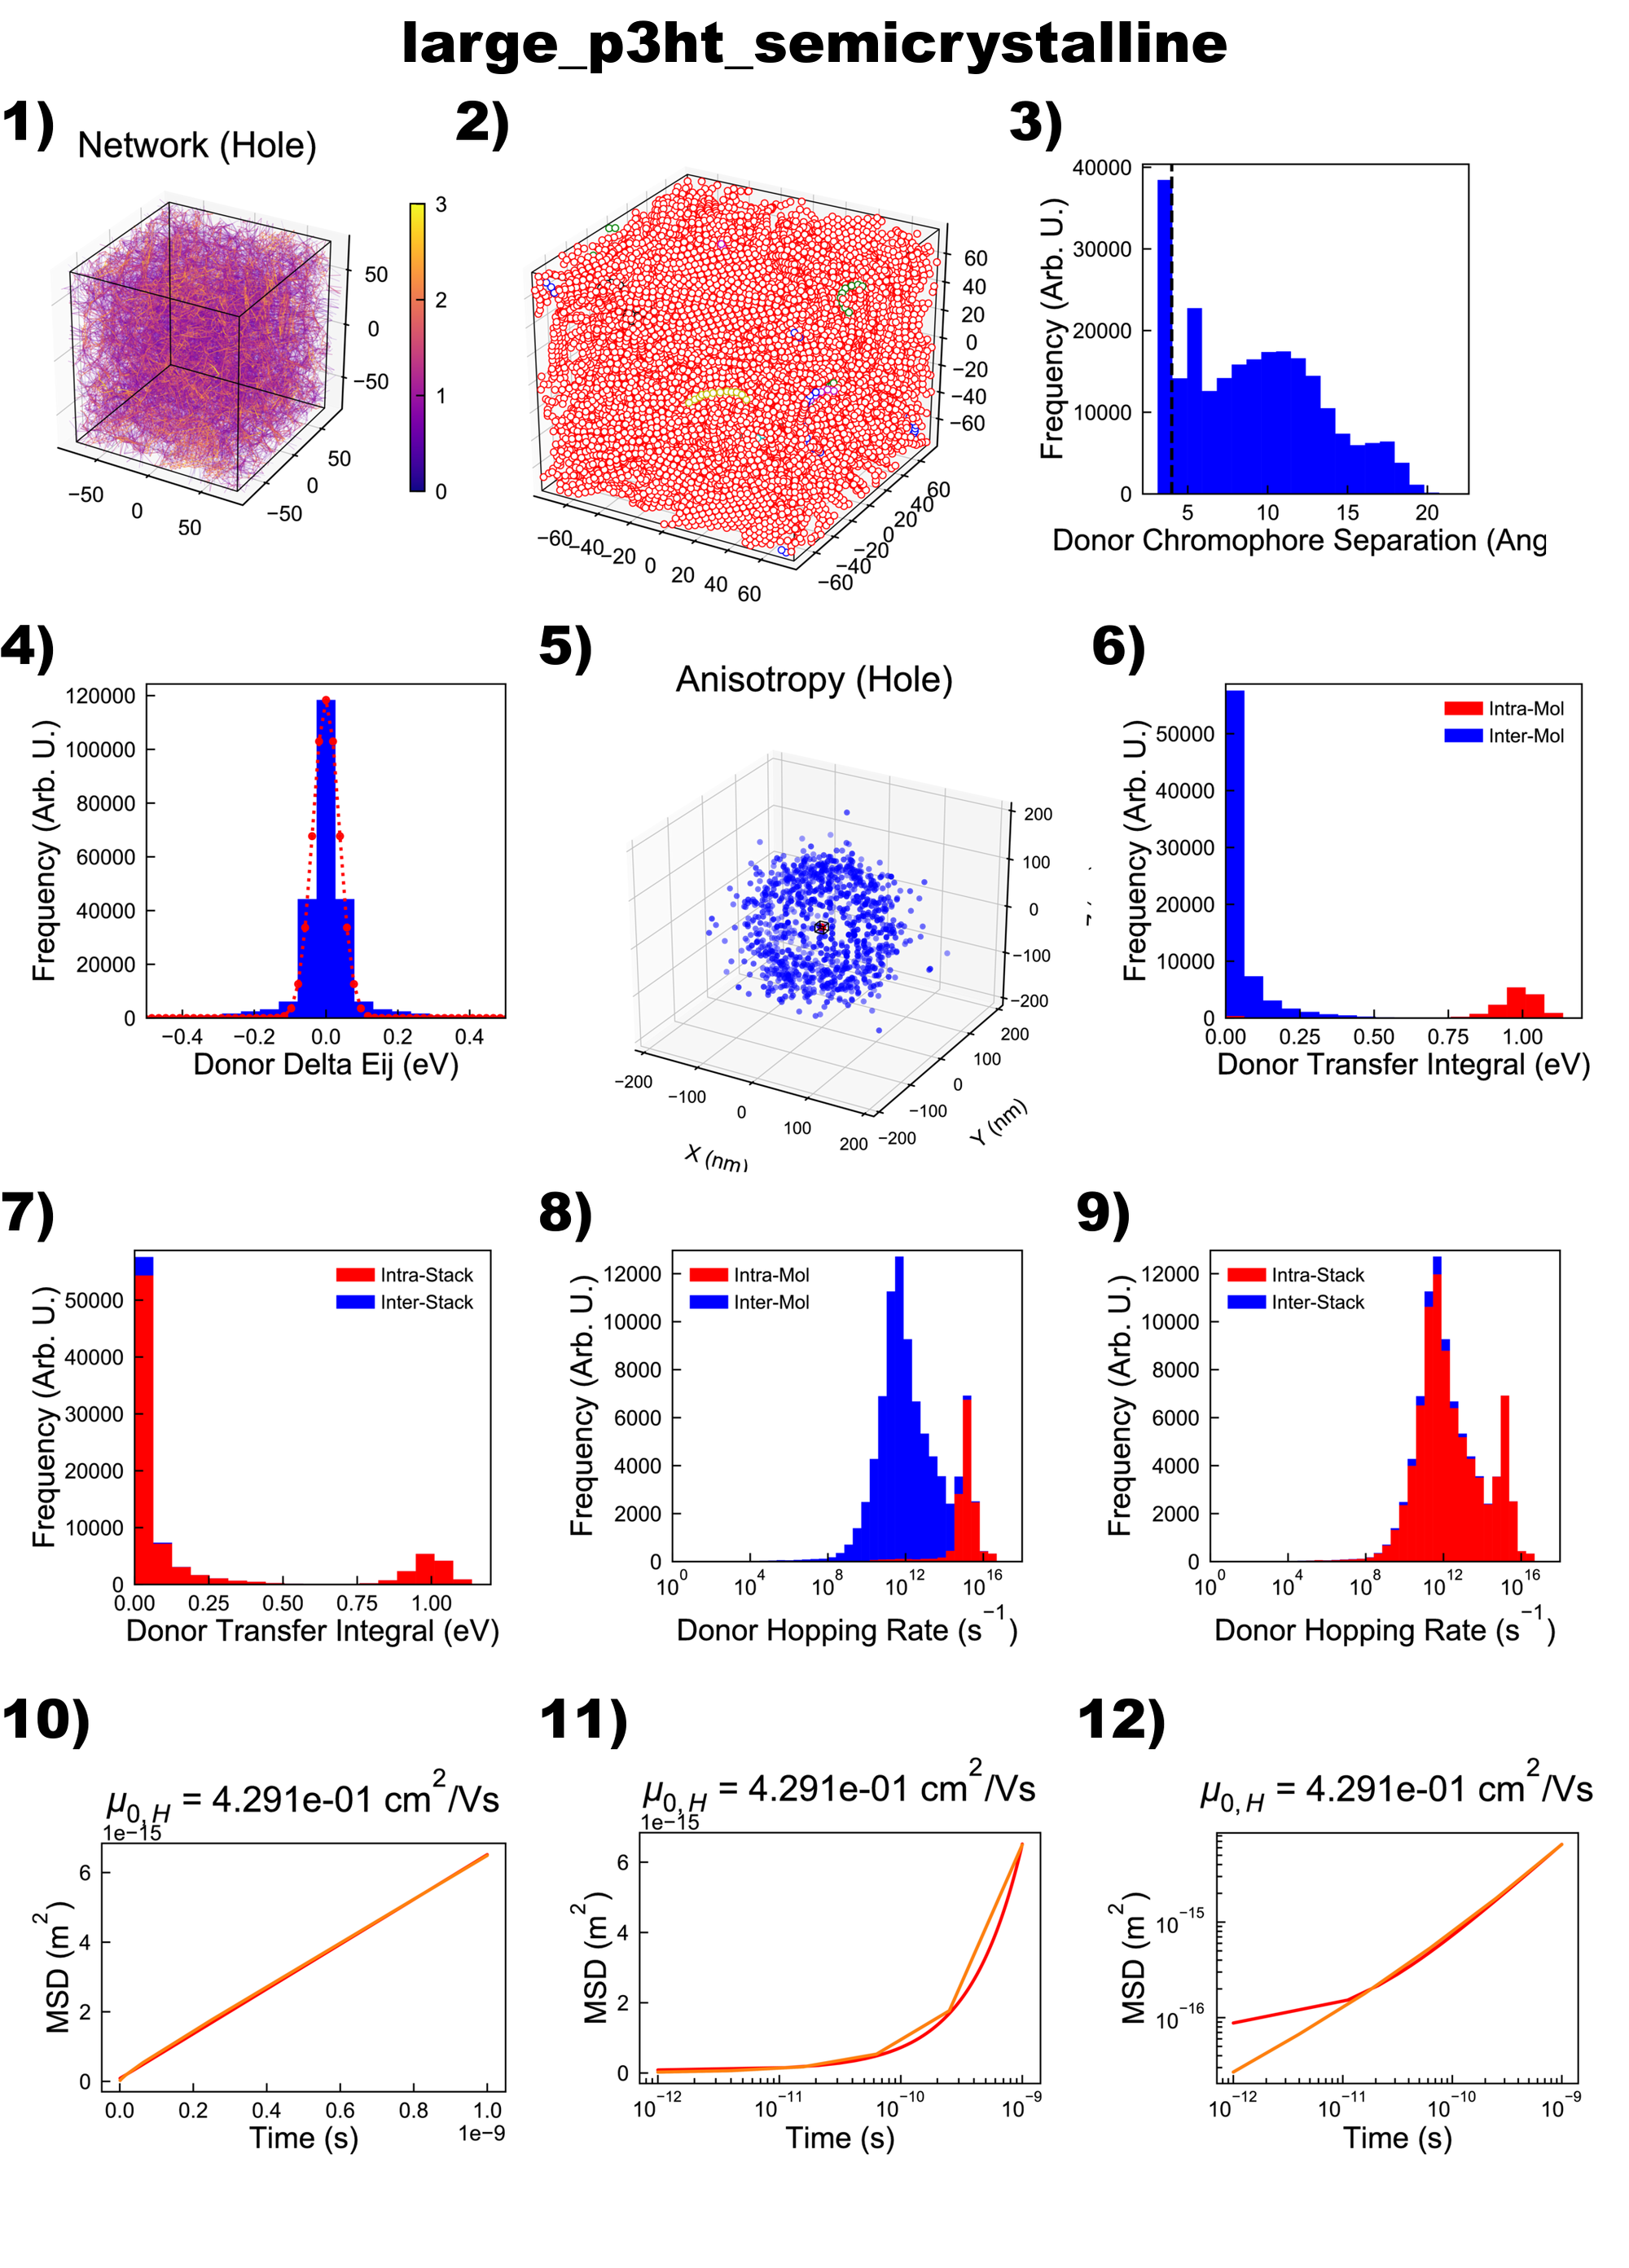
\includegraphics[width=0.85\textwidth]{Figures/large_p3ht_semicrystalline.png}
    \caption{   1) Chromophore connectivity network, 
                2) Location of `stacks', 
                3) Distribution of connected chromophore separations (defines stacks),
                4) Density of states of Frontier molecular orbital (delta Eij),
                5) KMC Carrier termination locations (defines anisotropy),
                6) Histogram of molecular transfer integrals,
                7) Histogram of stack transfer integrals,
                8) Histogram of molecular hopping rates,
                9) Histogram of stack hopping rates,
                10) Linear MSD plot,
                11) Semi-log-x MSD plot,
                12) Logarithmic MSD plot.}
	\label{fig:largeSemicrystalline}
\end{figure}


\begin{figure}[h]\centering
	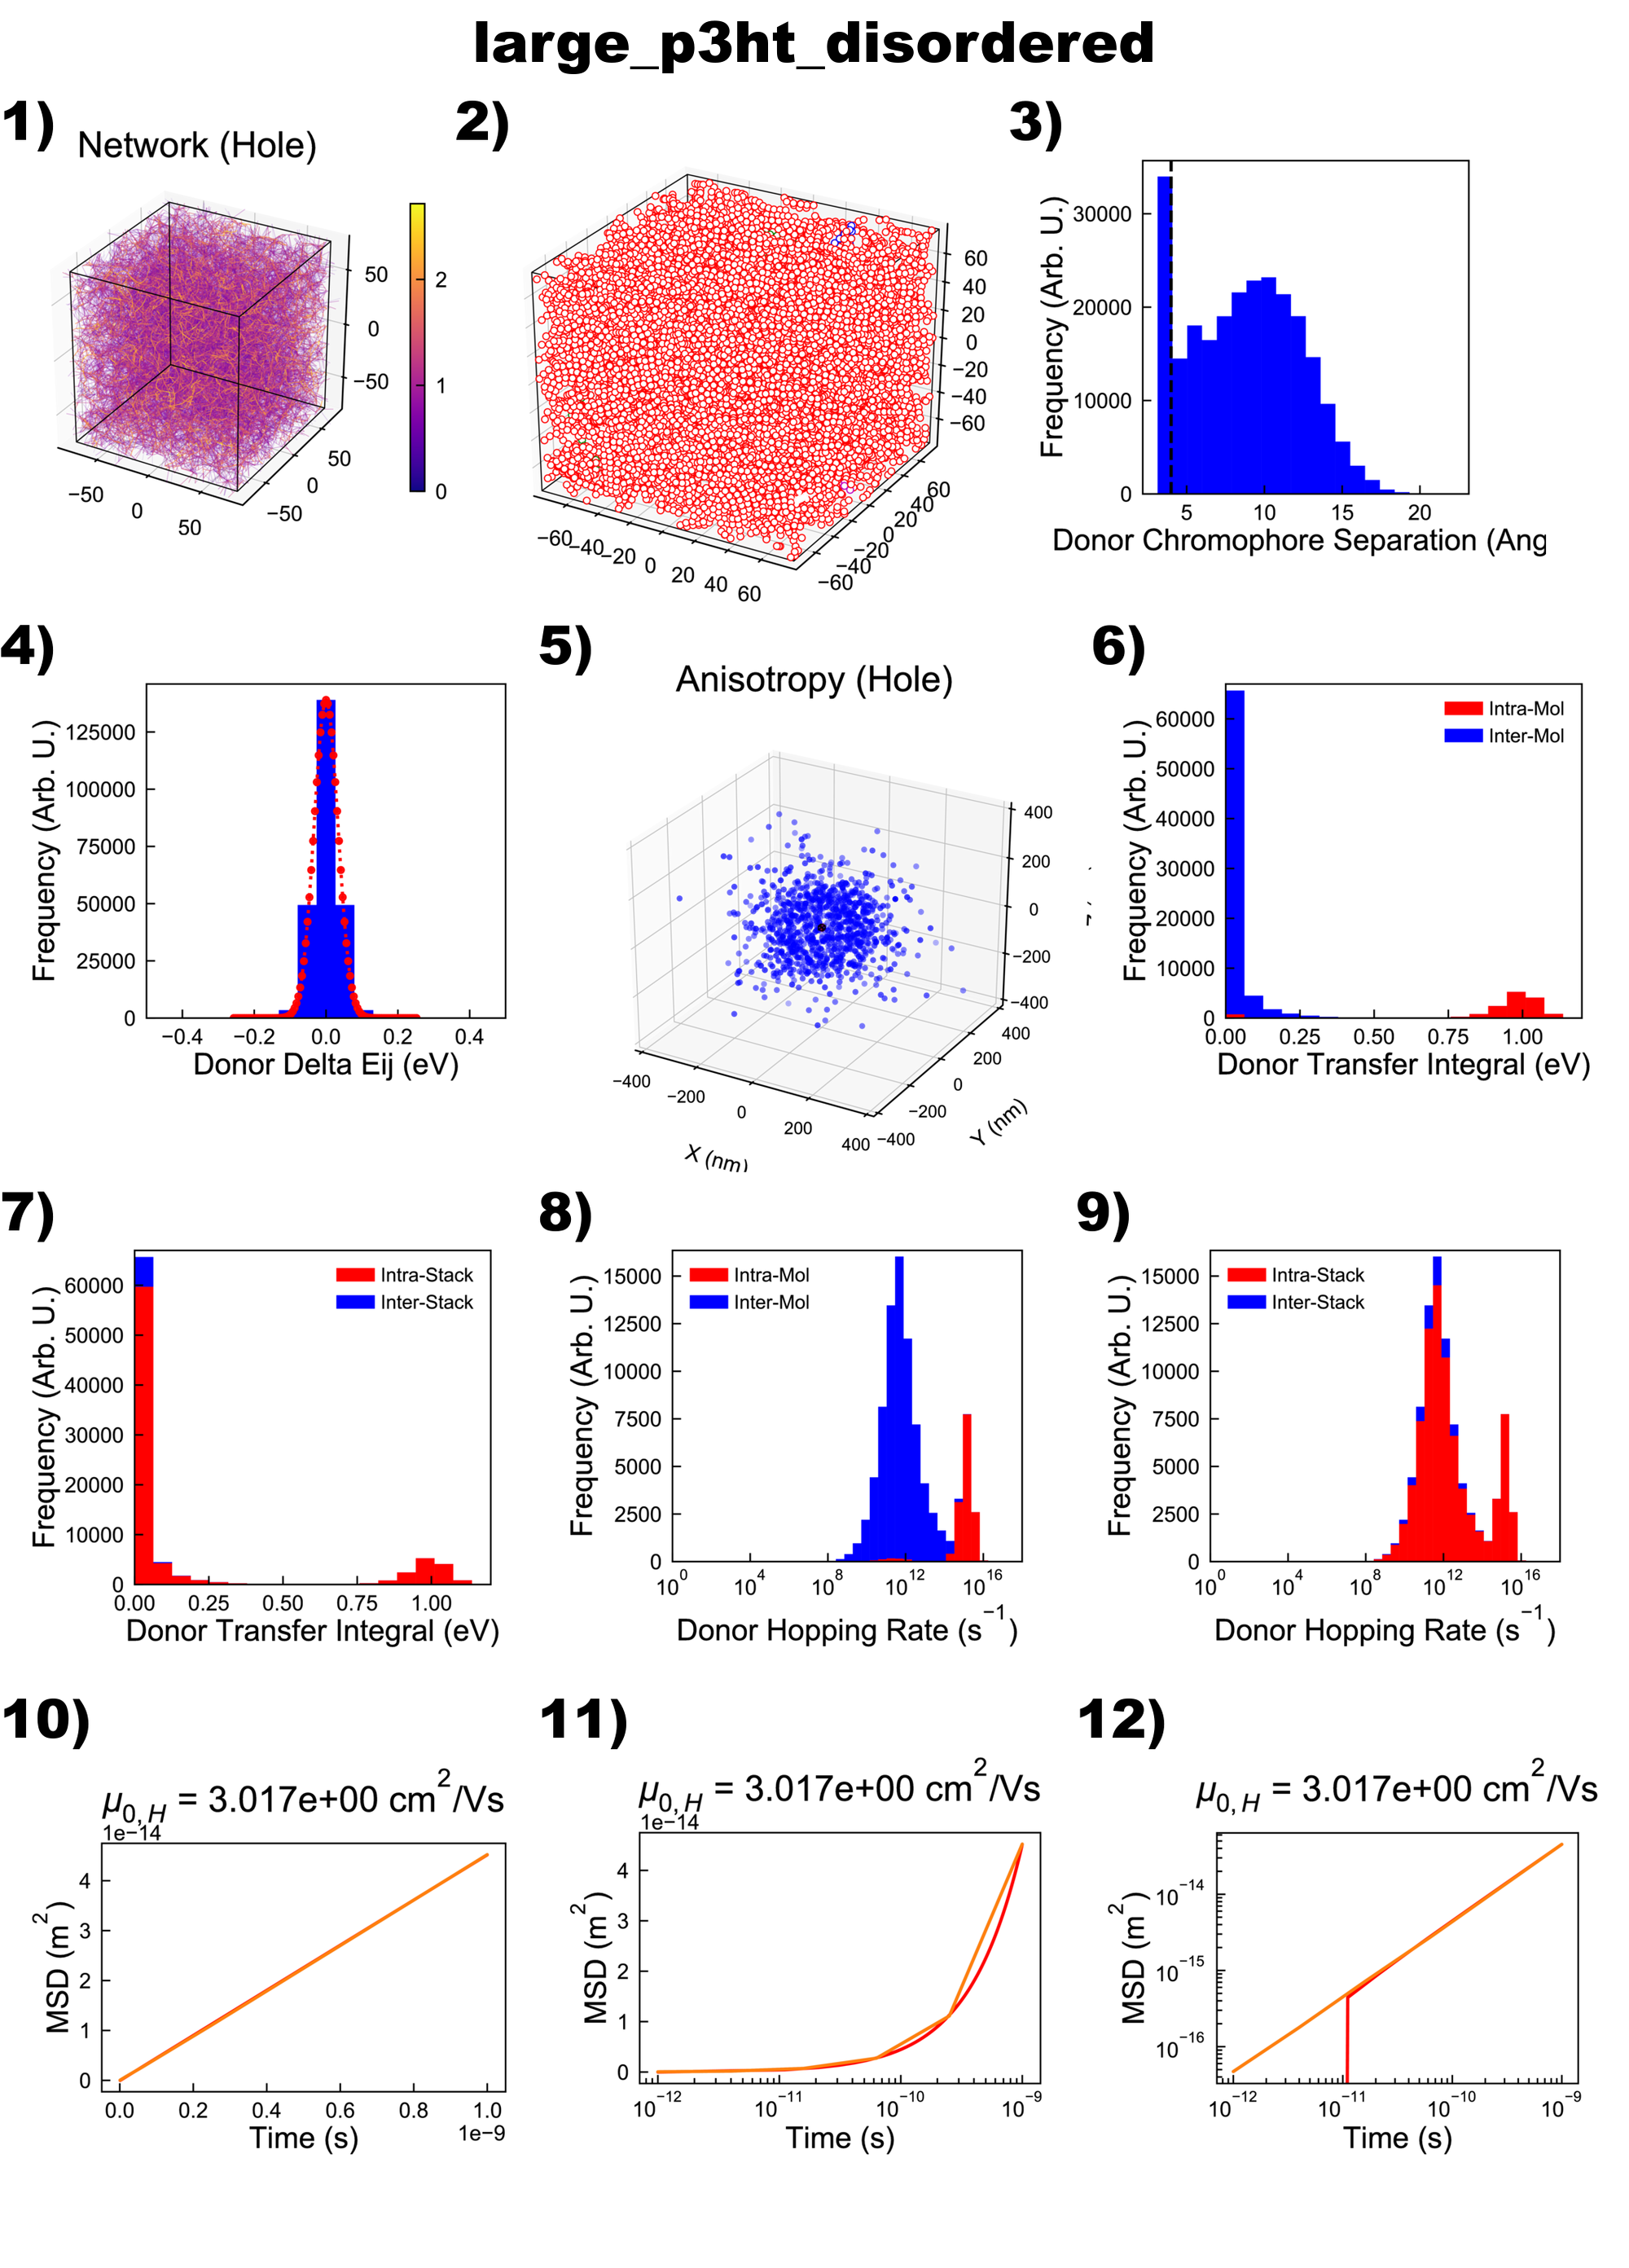
\includegraphics[width=0.85\textwidth]{Figures/large_p3ht_disordered.png}
    \caption{   1) Chromophore connectivity network, 
                2) Location of `stacks', 
                3) Distribution of connected chromophore separations (defines stacks),
                4) Density of states of Frontier molecular orbital (delta Eij),
                5) KMC Carrier termination locations (defines anisotropy),
                6) Histogram of molecular transfer integrals,
                7) Histogram of stack transfer integrals,
                8) Histogram of molecular hopping rates,
                9) Histogram of stack hopping rates,
                10) Linear MSD plot,
                11) Semi-log-x MSD plot,
                12) Logarithmic MSD plot.}
	\label{fig:largeDisordered}
\end{figure}


\begin{figure}[h]\centering
	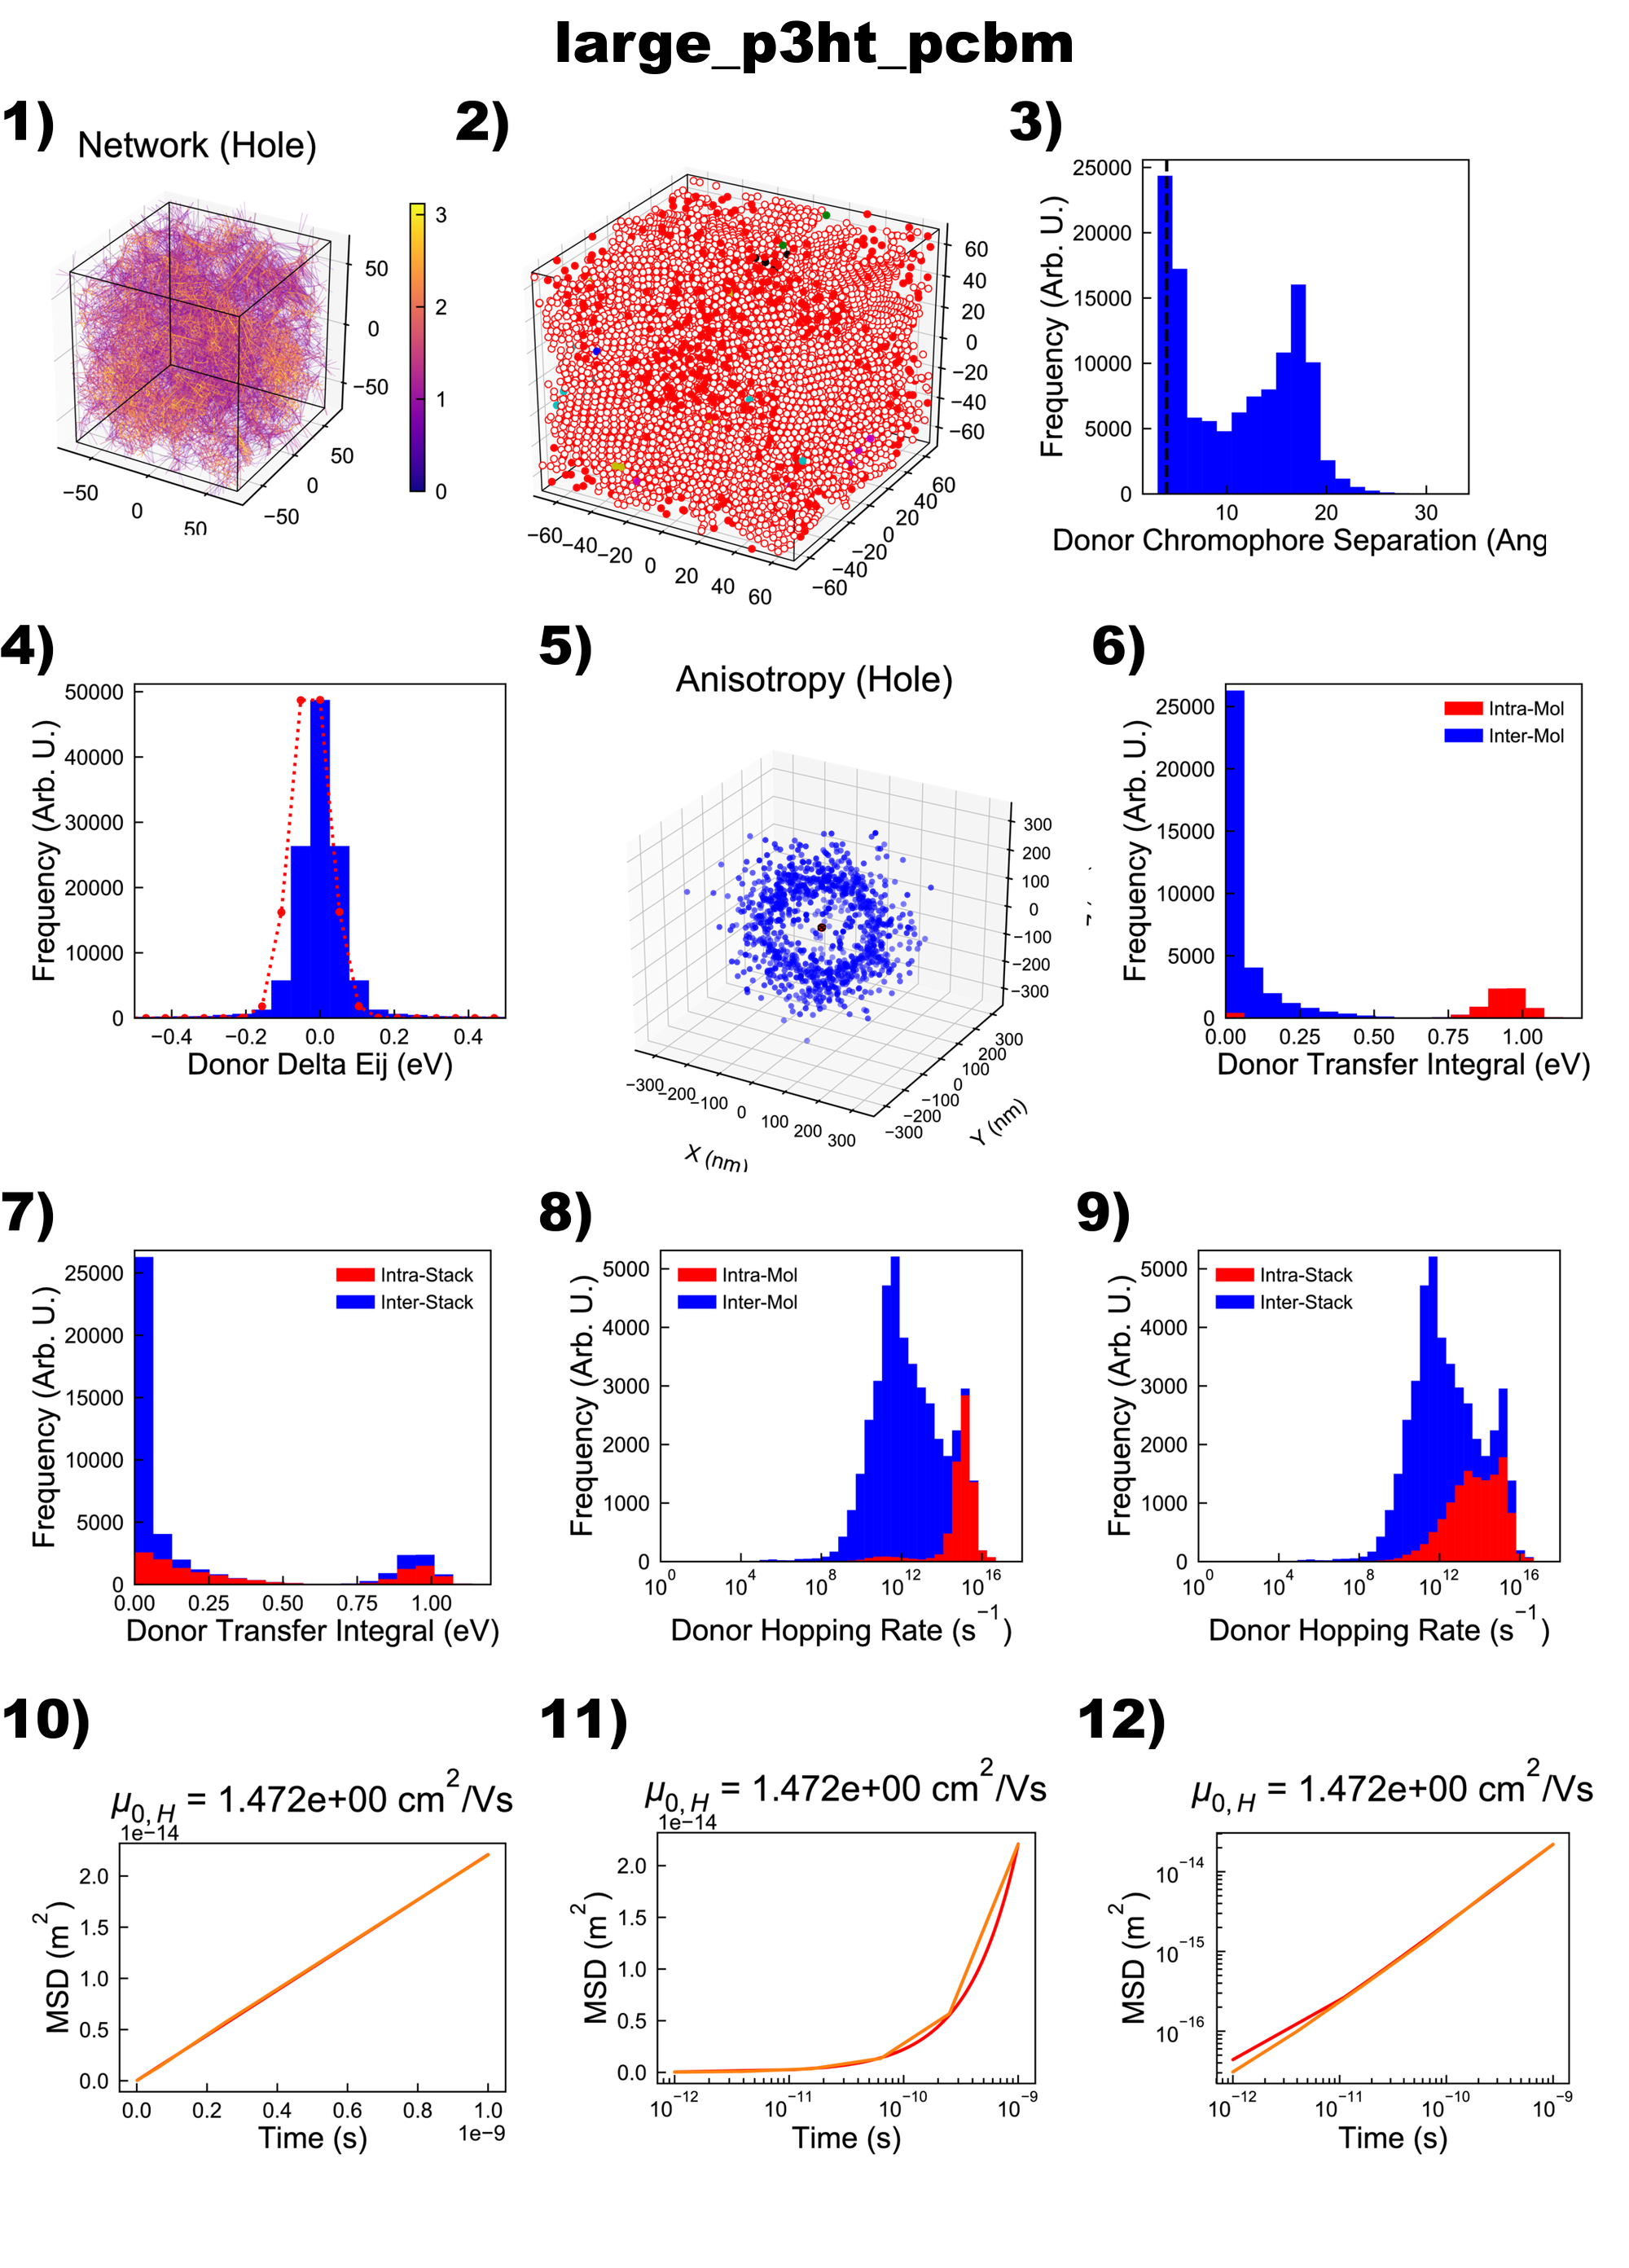
\includegraphics[width=0.85\textwidth]{Figures/large_p3ht_pcbm.png}
    \caption{   1) Chromophore connectivity network, 
                2) Location of `stacks', 
                3) Distribution of connected chromophore separations (defines stacks),
                4) Density of states of Frontier molecular orbital (delta Eij),
                5) KMC Carrier termination locations (defines anisotropy),
                6) Histogram of molecular transfer integrals,
                7) Histogram of stack transfer integrals,
                8) Histogram of molecular hopping rates,
                9) Histogram of stack hopping rates,
                10) Linear MSD plot,
                11) Semi-log-x MSD plot,
                12) Logarithmic MSD plot.}
	\label{fig:largePCBM}
\end{figure}


\bibliography{refs}
\bibliographystyle{unsrt}


\end{document}
